\documentclass{llncs}
\pdfoutput=1


\usepackage[utf8]{inputenc}
\usepackage[english]{babel}
%\usepackage[T1]{fontenc}
\usepackage{amsmath}
%\usepackage{amsthm}
\usepackage{amssymb}
\usepackage{hyperref}
\usepackage{braket}
%\usepackage[backend=biber,sortcites=true, maxcitenames=2, maxbibnames=99]{biblatex}
\usepackage{booktabs}
\usepackage{csquotes}
\usepackage{caption}
\usepackage{enumitem}
\usepackage{float}
\usepackage{graphicx}
\usepackage{hyperref}
\usepackage{mathdots}
\usepackage{mathtools}
\usepackage[linewidth=1pt]{mdframed}
\usepackage{microtype}
\usepackage{multicol}
\usepackage{physics}
\usepackage{pgfplots}
\usepackage{relsize}
\usepackage{rotating}
\usepackage{stmaryrd}   % doubled brackets
\usepackage{thmtools}
\usepackage{thm-restate}
\usepackage{tikzit}
In this section we provide a very brief explanation of what the ZX-calculus is and it's rewrite rules. For a more in depth overview of the ZX-calculus please refer to \cite{ZX-overview}.

\subsection{Generators}
The basic generator of the ZX-calculus are what we refer to as the \textit{spider}. There are two kinds of \textit{spiders}, the Z-spider and the X-spider. These spiders are then connected to each other by wires.

\todo {Completar a introducao ao ZX e regras de reescrita}
\usepackage{tikz}
\usepackage{todonotes}
%\usepackage[compact]{titlesec}
\usepackage{upgreek}
\usepackage[normalem]{ulem}
\usepackage{xargs} % Use more than one optional parameter in a new commands
\usepackage{xcolor}
\usepackage{xfrac}

\allowdisplaybreaks
\definecolor{zx_grey}{RGB}{211,211,211}
\definecolor{zx_red}{RGB}{232,165,165}
\definecolor{zx_green}{RGB}{216,248,216}

%\addbibresource{references.bib}




\begin{document}

%\title{An analysis of the Staggered Quantum Walk using the ZX-Calculus}
%\author{Bruno Jardim}
%\author{Luis Soares Barbosa}
%\affiliation{INESC TEC}
%

\title{Revisiting staggered quantum walks with ZX\thanks{This work was supported by FCT, the Portuguese Foundation for Science and Technology, within the project IBEX, with reference PTDC/CCI-COM/4280/2021.}}

%\title{An analysis of the Staggered Quantum Walk using the ZX-Calculus}
%
%\titlerunning{Bigraphical Modelling the Reconfiguration of Architectural Patterns}
\titlerunning{Deriving architectural reconfigurations}
%
\author{Bruno Jardim \inst{1} \and Jaime Santos\inst{1} \and Luis S. Barbosa \inst{1}}
%
\authorrunning{B. Jardim, J. Santos and L.S. Barbosa} 
%
\institute{
HASLab INESC TEC \& Universidade do Minho,\\ 
Campus de Gualtar, 4710-057 Braga, Portugal
%\email{pg49997@alunos.uminho.pt, jaimepereirasantos123@gmail.com, lsb@di.uminho.pt}
}


\maketitle

\begin{abstract}
    %Quantum Walks have a vast amount of applications in the current landscape of algorithm design. In this paper we analyse a specific implementation of a Quantum Walk, the Staggered Quantum Walk using the ZX-calculus. While conducting this analysis we discovered a possible alternative evolution operator for the Staggered Quantum Walk, that utilizes a much smaller amount of gates and can also be used in QPUs with limited qubit connectivity.
%
%
%Quantum walks, the quantum analogs of random walks, emerged as very versatile tool in quantum algorithm design, with exciting applications in unstructured search, graph algorithmics and communication protocols. Unlike their classical counterparts, they explore quantum interference patterns which, breaking the walk symmetry around the origin, leads to much quicker evolution of the walker, a sort of ballistic behaviour in the words of Venegas.
%


The staggered model is a recent, very general variant of discrete-time quantum walks which, avoiding the use of a coin to direct the walker evolution, explores the underlying graph structure to build an evolution operator based on local unitaries induced by adjacent vertices. Indeed, unlike conventional, coin-based quantum walks, which proceed straightforwardly from one vertex to another, the staggered variant takes advantage of forming partitions of graph cliques over the graph structure of the walking space. Then, it combines  local evolution operators  corresponding to different partitions  along discrete time steps.  Optimizing  the implementation of staggered walks in order to increase resilience to decoherence phenomena motivates their analysis with the ZX-calculus, an exercise that is the object of this short paper. As expected, the calculus rewrote the original circuit, significantly reducing the number of (expensive) gates used. Moreover, the exercise identified an underlying pattern leading to an alternative, potentially more efficient evolution operator.



%
%
%. Such a tessellation-based approach provides a
%structured framework for the evolution of quantum states, enabling the
%exploration of complex graph structures with enhanced versatility and
%precision~\cite{PhysRevA.98.052310,PhysRevA.98.012123}.  This model encompasses
%a substantial portion of the subclass of discrete-time quantum walks, including
%the coined and Szegedy's
%models~\cite{Portugal2016,Portugal2016_1,PhysRevA.95.012328}.
%
%
%
%
%Unlike their classical counterparts,
%quantum walks take advantage of quantum coherence, enabling interference
%effects that lead to the ballistic spreading of the walker. This unique
%characteristic has proven invaluable in various applications, from designing
%quantum search algorithms~\cite{PhysRevA.67.052307,Portugal2018} and
%implementing communication protocols~\cite{Shang_2018,8972594} to ac
%
%
%are a recent 
%quantum walks take advantage of quantum coherence, enabling interference
%effects that lead to the ballistic spreading of the walker. This unique
%characteristic has proven invaluable in various applications, from designing
%quantum search algorithms~\cite{PhysRevA.67.052307,Portugal2018} and
%implementing communication protocols~\cite{Shang_2018,8972594} to ac
\end{abstract}

\section{Introduction}
\label{sec:introduction}

Thought of as the quantum counterpart to classical random walks, quantum walks \cite{QW-overview} provide an interesting technique in algorithmic design, 
with  applications in unstructured search, graph algorithmics and communication protocols.

Differently from the classical case, where the  walker's next move follows the result of some sort of random choice, in a quantum setting evolution typically 
proceeds in an equally weighed superposition of possible moves through the iteration of a unitary operator, without resorting to intermediate measurements. 
This results in a very rich dynamics, in which the design of the evolution operator, and even seemingly
innocent differences  in its phase  and in the initial state, determine complex `walking patterns'  
which differ greatly both from each other and from the classical setting.

The relevance of quantum walks as a tool for algorithmic design justifies both a better understanding of their behaviour and the optimisation of their implementation, namely to increase resilience to decoherence phenomena. This  paper resorts to the ZX-calculus \cite{CoeckeD08,ZX-overview,CoeckeHKW22} for such a purpose. The ZX-calculus is a diagrammatic language for reasoning about linear maps between qubits. It is based on generators --- the \emph{spiders} --- that generalise rotations over the $Z$ and $X$ basis, and sets of rewrite rules whose completeness means that  equality between linear maps can be proven diagrammatically. This allows for program transformation in quantum software engineering, guided by powerful  circuit optimisation strategies for e.g. T-count reduction and gate compilation.

Optimisation of quantum circuits can be seen as a \emph{reconfiguration} process. Indeed, as shown in the following sections, the interpretation of such circuits as ZX-diagrams provides a flexible description of quantum computations graphically. Then, the rules of the ZX-calculus guide through a simplification strategy which corresponds to sequences of graph transformations. Finally, the reconfigured  circuit is extracted from the transformed graph. The process is illustrated here in a closed setting. However, it extends smoothly to the dynamic case as required by quantum algorithms which reconfigure themselves as a result of the (classical) evaluation of measurement results.  This is particularly relevant in the context of variational algorithms \cite{Cer21} which are core to current techniques in quantum machine learning \cite{Dun16}.



The exercise reported here focuses on a recent, very general variant of discrete-time quantum walks --- the \emph{staggered}
 model  \cite{PortugalSFG16} --- which, avoiding the use of a coin to direct the walker evolution, explores the underlying graph structure to build an evolution operator based on local unitaries induced by adjacent vertices.  The model is reviewed in Section 2. Then, in Section 3, its standard circuit implementation is translated and rewritten in ZX, supported by  the \textit{PyZX} tool \cite{pyzx}. This process leads in Section 4 to the identification of a diagrammatic pattern providing an interesting approximation to, and in some cases,  more efficient version, of the underlying evolution operator.  





\section{Staggered quantum walks}
\label{sec:staggered}
In contrast to conventional, coin-based quantum walks, which proceed straightforwardly from one vertex to another, the staggered variant  \cite{PortugalSFG16} takes advantage of forming partitions of graph cliques\footnote{A clique is a subset of vertices of an
undirected graph such that every two distinct vertices are adjacent.} over the graph structure of the walking space. Each partition forms a tesselation whose elements do not overlap. The set of
cliques in each tessellation must cover all vertices of the graph, and the set
of tessellations $\{T_{1}$,$T_{2}$, \ldots ,$T_{k}\}$ chosen
must cover all the edges.

Then  a unit vector, typically encoding a uniform
superposition, is associated to each clique so that
the vector belongs to the subspace spanned by the corresponding vertices; i. e., 
\begin{equation}
	\ket{u_{j}^{k}} = \frac{1}{\sqrt{\mathopen|\alpha_{j}^{k}}\mathclose|}\sum_{l\in\alpha_{j}^{k}}\ket{l},
\end{equation}
where $\alpha_{j}^{k}$ is the $j^{th}$ polygon in the $k^{th}$ tessellation.

This way each tessellation $k$ gives rise to an operator 
\begin{equation}
	H_k = 2\sum_{j=1}^{p}\ket{u_{j}^{k}}\bra{u_{j}^{k}} - I.
	\label{eq:StagHamil}
\end{equation}
which propagates the probability amplitude locally, in each clique.
The composition of all such operators defines the evolution operator, which, by solving the 
the time-independent Schr\"odinger equation, is equivalent to 
\begin{equation}
	U = e^{i\theta_{k}H_{k}}...e^{i\theta_{2}H_{2}}e^{i\theta_{1}H_{1}}, \text{  where  }\; e^{i\theta_{k}H_{k}} = \cos{(\theta_k)}I + i\sin{(\theta_k)}H_k
	\label{eq:stagWalkUnmodOp}
\end{equation}
since $H_k^2 = I$, meaning that the Hamiltonian is a reflection operator that,
when expanded in a Taylor series, generates a local operator.

As an elementary example consider a line where the following two tessellations  (depicted in red and blue below) are defined 
\begin{equation}
	T_{\alpha}= \{\{2x,2x+1\}\colon x \in \mathbb{Z}\}\; \; \text{and}\; \; T_{\beta}= \{\{2x+1,2x+2\}\colon x \in \mathbb{Z}\}.
\end{equation}

\begin{center}
	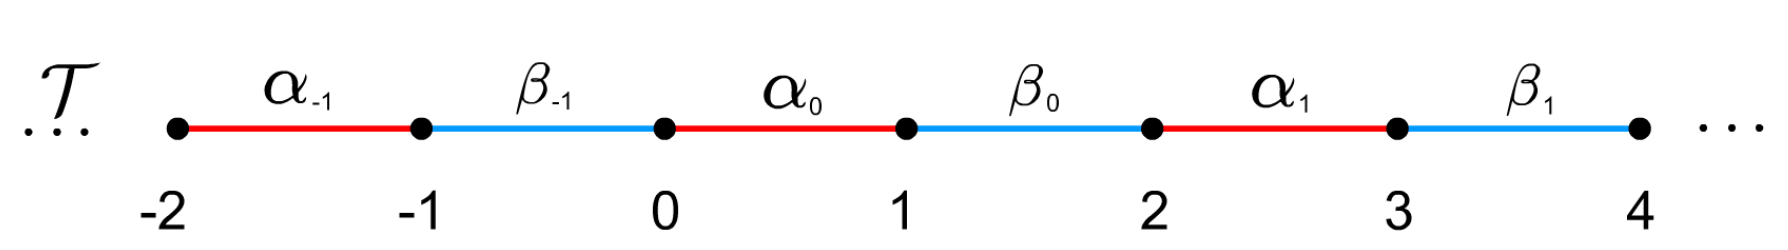
\includegraphics[scale=0.30]{img/tesselation.png}
\end{center}
Thus, 
\begin{equation}
	\ket{\alpha_x} = \frac{\ket{2x} + \ket{2x+1}}{\sqrt{2}}\; \; \text{and}\; \; \ket{\beta_x} = \frac{\ket{2x+1}+\ket{2x+2}}{\sqrt{2}},
\end{equation}
yielding Hamiltonians 
\begin{equation}
	H_\alpha = 2\sum_{x=-\infty}^{+\infty}\ket{\alpha_{x}}\bra{\alpha_x} - I \; \; \text{and}\; \;  H_\beta = 2\sum_{x=-\infty}^{+\infty}\ket{\beta_{x}}\bra{\beta_x} - I.
\end{equation}

Therefore, $U = e^{i\theta H_\beta}e^{i\theta H_\alpha}$ is the  evolution operator. The probability
distribution  on a line after 50 steps, starting at $\ket{+}$, for different values of $\theta$, is depicted below,    
noticing that the walker is more likely to be found further away from the origin
as the angle increases.
\begin{center}
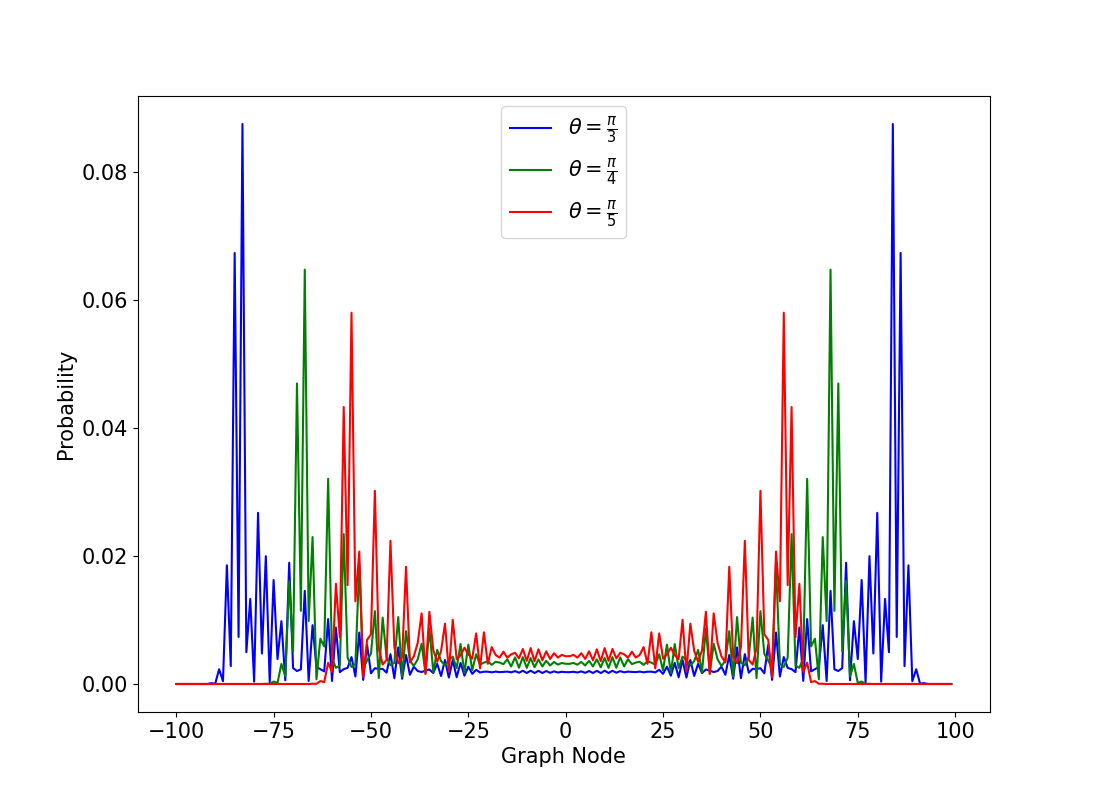
\includegraphics[scale=0.30]{img/stagqwMultiple.png}
\end{center},



%\section{ZX-calculus}
%\label{sec:zx-calculus}
%In this section we provide a very brief explanation of what the ZX-calculus is and it's rewrite rules. For a more in depth overview of the ZX-calculus please refer to \cite{ZX-overview}.

\subsection{Generators}
The basic generator of the ZX-calculus are what we refer to as the \textit{spider}. There are two kinds of \textit{spiders}, the Z-spider and the X-spider. These spiders are then connected to each other by wires.

\todo {Completar a introducao ao ZX e regras de reescrita}

\section{Bringing ZX into the picture}
\label{sec:sqw}


A circuit implementation of the staggered model can be found in \cite{MScJaime}. As expected, it resorts to the joint tessellation dynamics, in contrast to a coined quantum walk that uses a coin as a shift operator. For the example discussed above, it yields
\ctikzfig{sqw-circuit}
where $R_x(\theta) = e^{\frac{-i\theta X}{2}}$ and the Inc(rement) and Dec(rement) circuits have the usual implementation through  generalised Toffoli gates. When the walker reaches the limit of the state space it cycles back.
An  implementation for a 3 qubit staggered quantum walk, and taking $\theta = \frac{\pi}{3}$, which maximizes\footnote{For this specific graph $\theta = \frac{\pi}{3}$ maximizes propagation, however $\frac{\pi}{2}$ is the optimal parameter for a complete graph.} propagation, is represented in a ZX diagram as

\begin{align*}
    \tikzfig{1-step-sqw}
\end{align*}
\captionof{figure}{A ZX-diagram of a 1-step staggered quantum walk with the starting state $\ket{4}$, that being the reason for the $\pi$ X-spider on the third qubit.}
~\\

\noindent
which takes advantage of the ZH-calculus H-box notation for representing Toffoli gates in a concise way. Expanding Toffoli into its basic gates leads to 

\begin{align*}
    \tikzfig{1-step-expanded}
\end{align*}
~\\

Some simple optimisations can be considered to deal with the CNOT gate at the end of the expansion of the Toffoli gate and the CNOT belonging to the increment operator, and similarly, but for a X-spider between the CNOT targets,  in the decrement operator. Moreover, one may cancel the two X-spiders with phase $\pi$ in the first qubit between the increment and decrement layers, and the two consecutive Hadamard gates in the last qubit. The result is 
the following ZX-diagram,

\begin{align*}
    \tikzfig{1-step-trivial}
    \label{fig:trivial}
\end{align*}
~\\

These optimisations  slightly reduced the number of Clifford gates in the diagram. More advanced techniques, described in \cite{t-count-opt} and  directly implemented in \textit{PyZX} \cite{pyzx} as the \texttt{full\_reduce} method, may reduce the circuit T-count  in about $50\%$ \cite{t-count-opt}. Although this is not the case for our small example, when we start applying such simplifications to staggered models with  larger amounts of steps the T-count reduction can reach  approximately $60$-$70\%$.
Back to the example, this simplification yields 

\begin{align*}
    \tikzfig{graph-like}
\end{align*}
~\\

This diagram no longer resembles a circuit, making a comparison with the original one difficult. The circuit extracted \cite{extraction-p-hard} by \textit{PyZX} has 
more gates than the one obtained from the simple optimisations mentioned above,  although the T-count is indeed smaller.
  
%\begin{align}
%    \tikzfig{fullreduce-simple}
%\end{align}

In fact, the \texttt{full\_reduce} method introduces several additional Hadamard gates  to make all the edges Hadamard-edges, and color-changes all the X-spiders. 
The subsequent  circuit extraction  'preserves' the nature of the \textit{graph-like} ZX-diagram. As such there are a lot of Hadamard gates and Z-spiders that could cancel-out or change color. Following the extraction with a small set of simplifications, basically resorting to fusion rewrite rules followed by a color-change, we get a much smaller circuit. 

This fully-simplified circuit now surpasses the original circuit in both the total amount of gates and T-count, but not the one obtained with the simple optimisations above. Although the reduction of both these metrics are not that significant in this example, when applying the same techniques in models with a greater number of steps  reductions in the number of gates and T-count become quite clear. The following tables show, respectively, the total number of  gates and the T-count value induced by the different optimisation procedures used on the same 3-qubit implementation.

\begin{table}[H]
\centering
\begin{tabular}{|l|cccc|}
\hline
                               & \multicolumn{4}{l|}{Number of steps in the staggered quantum walk:}                                   \\ \hline
Optimizations used:          & \multicolumn{1}{c|}{1}  & \multicolumn{1}{c|}{2}  & \multicolumn{1}{c|}{4}   & 8   \\ \hline
None            & \multicolumn{1}{c|}{39} & \multicolumn{1}{c|}{77} & \multicolumn{1}{c|}{153} & 305 \\ \hline
Simple     & \multicolumn{1}{c|}{31} & \multicolumn{1}{c|}{59} & \multicolumn{1}{c|}{115} & 227 \\ \hline
Full-reduce + fusion/id/to\_rg & \multicolumn{1}{c|}{37} & \multicolumn{1}{c|}{47} & \multicolumn{1}{c|}{72}  & 118 \\ \hline
\end{tabular}

%\label{tab:total-gates}
\end{table}
\caption{Number of total gates in the circuit in relation to the simplification routines used}
%\vspace{-1cm}
\begin{table}[H]
\centering
\begin{tabular}{|l|cccc|}
\hline
                               & \multicolumn{4}{l|}{Number of steps in the staggered quantum walk:}                                  \\ \hline
Optimizations used:          & \multicolumn{1}{c|}{1}  & \multicolumn{1}{c|}{2}  & \multicolumn{1}{c|}{4}  & 8   \\ \hline
None            & \multicolumn{1}{c|}{16} & \multicolumn{1}{c|}{32} & \multicolumn{1}{c|}{64} & 128 \\ \hline
Simple       & \multicolumn{1}{c|}{16} & \multicolumn{1}{c|}{32} & \multicolumn{1}{c|}{64} & 128 \\ \hline
Full-reduce + fusion/id/to\_rg & \multicolumn{1}{c|}{10} & \multicolumn{1}{c|}{16} & \multicolumn{1}{c|}{28} & 52  \\ \hline
\end{tabular}
\end{table}
\caption{T-count in the circuit in relation to the simplification routines used}
%The Staggered Quantum Walk is already suitable for the current NISQ landscape \cite{MScJaime}, with these simplification routines we can minimize even further noise induced errors and decoherence.












\section{An alternative evolution operator}
\label{sec:ev-op}
When analyzing the resulting circuit of longer ($\ge$ 5 steps) SQWs a pattern starts to emerge in the resulting circuit. This pattern also is repeated in the same amount as the number of steps in the quantum walk. This leads us to believe that this operator is capable of representing both the increment and decrement layers of the evolution operator, or at least approximate the SQW evolution operator.

The following is a ZX-diagram representation of the above-mentioned operator.

\begin{align}
    \tikzfig{sqw-pattern-standard}
\end{align}

Where:

\begin{equation}
    \alpha_n = \pm \frac{\pi}{4}
\end{equation}
\begin{equation}   
    \beta_n = \frac{2\pi}{3} + n\pi 
\end{equation}

with $n=0$ or $n=1$.


There is also a slight variation of this operator, where a CNOT gate between the first and last qubit appears right after the $\beta_1$ Z-spider.


\begin{align}
    \tikzfig{sqw-pattern-variation}
\end{align}

This operator by itself doesn't fully capture the SQW we started with, but in conjunction with a set of gates in the beginning and the end of the circuit it represents the exact same tensor as the original circuit. 


% Possivelmente utilizar o seguinte para as desvantagens

These initial and final set of gates do not seem to follow any sort of structure or reason for the gates that are used. However, the initial segment of the circuit always appears to have 4 rotations combined with a seemingly random arrangement of other phase-less gates.


This operator appeared when optimizing the 3 qubit Staggered Quantum Walk, however if one follows the way this operator is constructed this can be generalized for an $n$ qubit implementation of this operator.

Thus yielding the following operator, in the form of a ZX-diagram:

\begin{align}
    \tikzfig{sqw-pattern-generalization}
\end{align}

This operator is constructed by entangling the first and last qubit and placing them in superposition. This is achieved by the XCX-gate (which is a CNOT with an hadamard on both sides of the control), then it is followed by a CNOT gate between the first and last qubit and a rotation over the X-axis on the first qubit. Afterwards a ladder of XCX-gates starting with the first qubit and the $n-1^{th}$ qubit and descending all the way to the second. This is then followed by a rotation over the Z-axis along with a X-axis rotation. Then a CNOT is applied to the first and last qubit, following this there's a X-axis rotation and a XCX-gate over the first qubit and the $n-1^{th}$ qubit. Then there's the second Z-axis rotation subsequently followed by the same ladder of XCX-gates, although this time it starts between the first and the $n-2^{th}$ qubit and descending all the way to the second. Finishing off with the last X-axis rotation.

The logic behind this operator is creating an uniform distribution over a certain number of states, applying a rotation to that uniform distribution that makes some states more likely than others and then spreading these probabilities over the other states using CNOT gates.

When we take the nature of this operator into consideration it is obvious why it only shows up in SQWs over a certain length. The classical operator for the SQW using the increment and decrement layers needs to be repeated a number of times to be able to spread the probabilities distribution over the whole state space. This is something that this alternative operator does on the first layer, thus it cannot approximate SQWs with a small number of steps as well as it can for longer quantum walks.

\subsection{Advantages of this alternative operator}

Besides this this new operator has a whole set of advantages. The first one being the total amount of gates needed to represent the evolution of the quantum walk. With the number of qubits in the SQW increasing so does the the cost of the increment and decrement layers, as a $n$ qubit SQW needs to implement MCX gates with $n-1$ controls. These MCX gates need to then be expanded into it's basic gates representation \cite{gate-decomp}. All the while this new operator at most utilizes gates controlled with at most 1 qubit. Also when we go from a $n$ qubit to a $n+1$ qubit quantum walk all that needs to be done is add two more XCX-gates, one to each ladder of XCX-gates, the same can't be said about the evolution operator based on increment and decrement operators. 

This leads to this alternative operator being much more efficient when it comes to the total amount of gates used, leading to lower depth circuits and in turn less error prone.



Just by itself this operator is capable of approximating the evolution of a SQW. Although the approximation isn't perfect it can yield results with a distribution of probabilities quite similar to the original implementation of the SQW.

\todo {Graficos a comparar}

One particular advantage of this specific implementation of the evolution operator is that it can work quite well on QPUs that have a very limited connectivity. This is due to the fact that all the qubits used in the SQW only need to have a strong connectivity with only the first qubit, thus minimizing possible errors occurring from having to operate on two qubits with poor connectivity.

\subsection{Disadvantages of this alternative operator}

Although this operator presents itself with a plethora of advantages it also presents a lot of challenges when it comes to actually using it. This is due mostly to the lack of reason as to which values should the $\alpha_n$ and $\beta_n$ parameters be. Or even, if these parameters should change with the change of how many qubits are used in the Staggered Quantum Walk. When optimizing the 3 qubit implementation of the SQW the resulting parameters did not seem to follow any reasonable pattern. 

There doesn't seem to be a way to determine which values these parameters should take to approximate a given SQW.

Also, there doesn't seem to be a guarantee as to if the next step of the SQW will be able to be approximated with the already established parameters, this can lead to sub-par approximations of the Staggered Quantum Walk.













\section{Conclusions and future work}
\label{sec:conclusion}
In this article we studied how the Staggered Quantum Walk behaves when subjected to the circuit optimization routines that the ZX-calculus offers us. We've shown that the current implementations of the Staggered Quantum Walk can be heavily optimized in both the total number of gates and the T-count. With both of them capable of reaching a reduction of 60-70\% in both of these metrics. Making the SQW an even stronger candidate for NISQ algorithms.

We have also introduced a possible alternative operator to the evolution operator of the Staggered Quantum Walk, being this operator much smaller in the number of total gates and capable of being run on certain, more limited, QPUs.

However, this operator is not without its challenges. It is very non-trivial to use and the problem of which rotations $\alpha_n$ and $\beta_n$ that should be used is far from being solved. Formalizing these rotations would be a necessary step for using this operator conveniently.

Also, the initial state of the quantum walk influences how well the operator approximates the SQW, e.g., if we construct a number of layers of the operator such that it approximates a 5 step SQW with $\ket{4}$ as the initial state, those same layers most likely won't approximate a 5 step SQW with, for example, $\ket{2}$ as the initial state.

In the particular case of the 3 qubit implementation of the SQW it remains an open question what is happening in the initial and final set of seemingly random gates is, for these are the reason the resulting circuit represents the exact same tensor product as the original one.

When applying the exact same circuit simplification routines to a 4 qubit implementation of the Staggered Quantum Walk, this operator did not appear in the resulting circuit. In fact, contrary to the 3 qubit implementation the resulting circuit did not have any sort of structure, it was mostly a seemingly random arrangement of gates.








\bibliographystyle{alpha}
\bibliography{references.bib}

% \newpage
%\printbibliography



\end{document}